\chapter{Gated Recurrent Units (GRU) \cite{dnn-1}}


\begin{figure}[H]
    \centering
    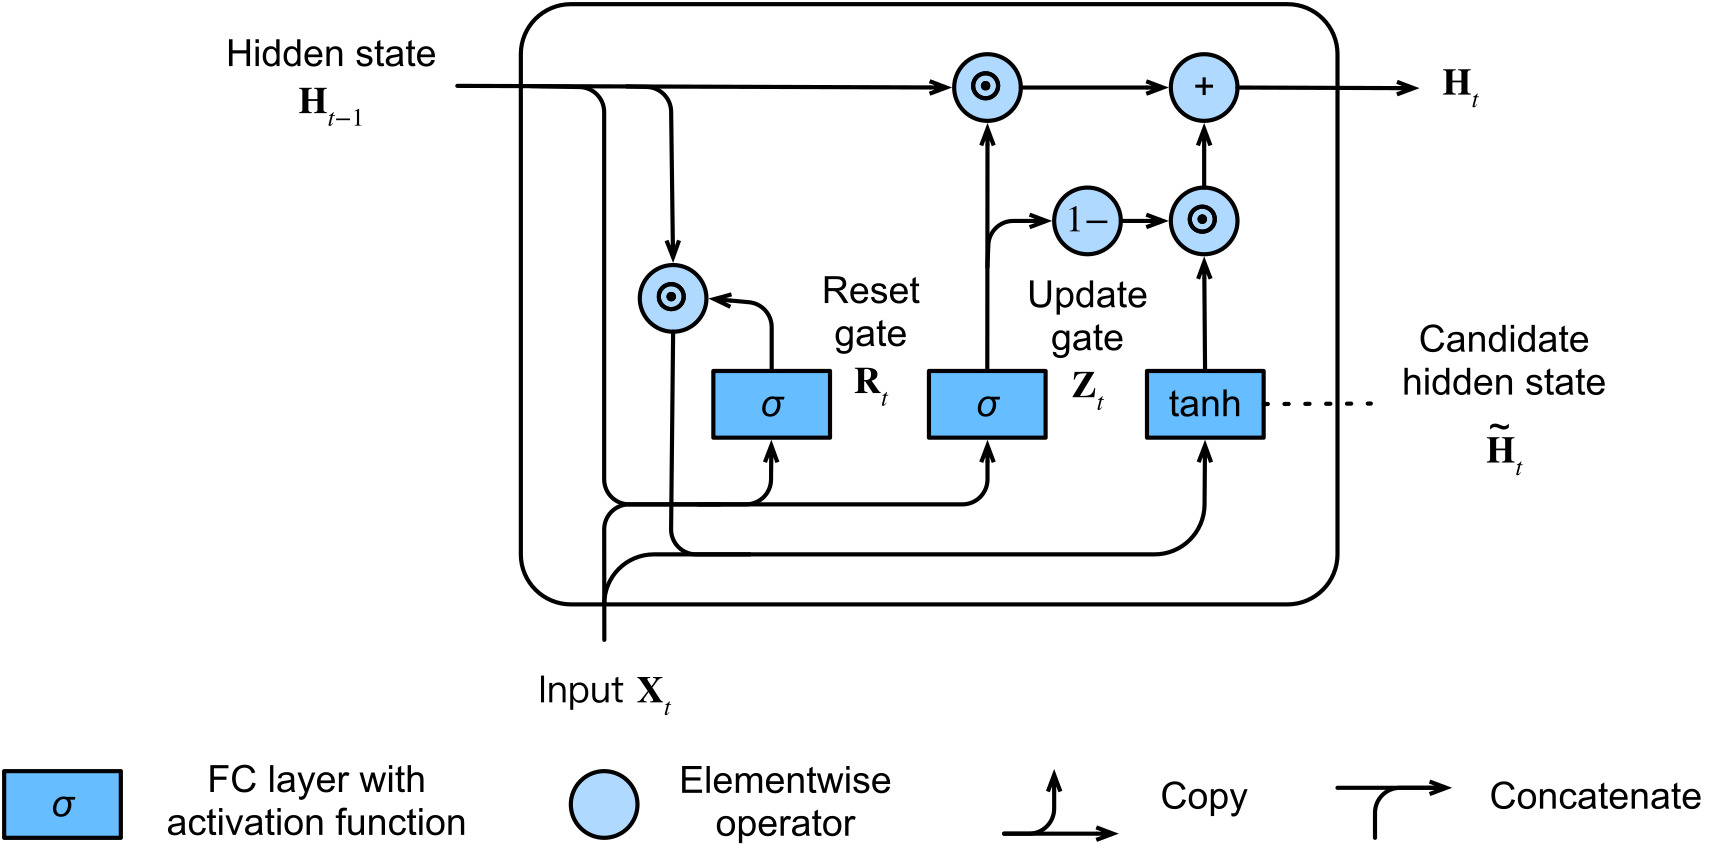
\includegraphics[width=\linewidth, height=5cm, keepaspectratio]{Pictures/Gated-Recurrent-Units/gru-final.jpg}
\end{figure}


\begin{customTableWrapper}{1.5}
\begin{longtable}{l l p{8cm}}
    \hline
    \customTableHeaderColor
    \multicolumn{3}{c}{Inputs} \\ \hline

    $t$ & $\in \mathbb{R}$ & time step \\
    $n$ & $\in \mathbb{R}$ & number of examples\\
    $d$ & $\in \mathbb{R}$ & number of inputs \\
    $\mathbf{X}_t$ & $\in \mathbb{R}^{n \times d}$ & input (minibatch) \\

    \hline
    \customTableHeaderColor
    \multicolumn{3}{c}{Hidden State} \\ \hline

    $h$ & $\in \mathbb{R}$ & number of hidden units \\
    $\mathbf{H}_{t-1}$ & $\in \mathbb{R}^{n \times h}$ & hidden state of the previous time step \\
    $\mathbf{H}_t$ & $\in \mathbb{R}^{n \times h}$ & new hidden state \\
    
    \hline
    \customTableHeaderColor
    \multicolumn{3}{c}{Reset Gate} \\ \hline

    $\mathbf{W}_{\textrm{xr}}$ & $\in \mathbb{R}^{d \times h}$ & weight parameter \\
    $\mathbf{W}_{\textrm{hr}}$ & $\in \mathbb{R}^{h \times h}$ & weight parameter \\
    $\mathbf{b}_\textrm{r}$ & $\in \mathbb{R}^{1 \times h}$ & bias parameter \\
    $\mathbf{R}_t$ & $\in \mathbb{R}^{n \times h}$ & reset gate \\

    \hline
    \customTableHeaderColor
    \multicolumn{3}{c}{Update Gate} \\ \hline

    $\mathbf{W}_{\textrm{xz}}$ & $\in \mathbb{R}^{d \times h}$ & weight parameter \\
    $\mathbf{W}_{\textrm{hz}}$ & $\in \mathbb{R}^{h \times h}$ & weight parameter \\
    $\mathbf{b}_\textrm{z}$ & $\in \mathbb{R}^{1 \times h}$ & bias parameter \\
    $\mathbf{Z}_t$ & $\in \mathbb{R}^{n \times h}$ & update gate \\

    \hline
    \customTableHeaderColor
    \multicolumn{3}{c}{Candidate Hidden State} \\ \hline
    $\mathbf{W}_{\textrm{xh}}$ & $\in \mathbb{R}^{d \times h}$ & weight parameter \\
    $\mathbf{W}_{\textrm{hh}}$ & $\in \mathbb{R}^{h \times h}$ & weight parameter \\
    $\mathbf{b}_\textrm{h}$ & $\in \mathbb{R}^{1 \times h}$ & bias parameter \\
    $\tilde{\mathbf{H}}_t$ & $\in \mathbb{R}^{n \times h}$ & candidate hidden state \\


\end{longtable}
\end{customTableWrapper}



\begin{enumerate}
    \item The gated recurrent unit (GRU) offered a streamlined version of the LSTM memory cell that often achieves comparable performance but with the advantage of being faster to compute

    \item 
\end{enumerate}



\section{Components of GRU \cite{dnn-1}}

\begin{enumerate}[itemsep=0.15cm]
    \item \textbf{Reset Gate}
    \begin{enumerate}
        \item $\mathbf{R}_t = \sigma(\mathbf{X}_t \mathbf{W}_{\textrm{xr}} + \mathbf{H}_{t-1} \mathbf{W}_{\textrm{hr}} + \mathbf{b}_\textrm{r})$
        
        \item this gate is given sigmoid activations, forcing its values to lie in the interval $(0,1)$

        \item reset gate controls how much of the previous state we might still want to remember

        \item Reset gates help capture \textbf{short-term} dependencies in sequences
    \end{enumerate}
    
    \item \textbf{Update Gate}
    \begin{enumerate}
        \item $\mathbf{Z}_t = \sigma(\mathbf{X}_t \mathbf{W}_{\textrm{xz}} + \mathbf{H}_{t-1} \mathbf{W}_{\textrm{hz}} + \mathbf{b}_\textrm{z})$

        
        \item this gate is given sigmoid activations, forcing its values to lie in the interval $(0,1)$

        \item update gate would allow us to control how much of the new state is just a copy of the old one

        \item This determines the extent to which the new hidden state $\mathbf{H}_t$ matches the old state $\mathbf{H}_{t-1}$ compared with how much it resembles the new candidate state $\tilde{\mathbf{H}}_t$

        \item Whenever the update gate $\mathbf{Z}_t$ is close to 1, we simply retain the old state\\
        In this case the information from $\mathbf{X}_t$ is ignored, effectively skipping time step $t$ in the dependency chain

        \item whenever $\mathbf{Z}_t$ is close to 0, the new latent state $\mathbf{H}_t$ approaches the candidate latent state

        \item Update gates help capture \textbf{long-term} dependencies in sequences
    \end{enumerate}

    \item \textbf{Candidate hidden state}
    \begin{enumerate}
        \item $\tilde{\mathbf{H}}_t = \tanh(\mathbf{X}_t \mathbf{W}_{\textrm{xh}} + \left(\mathbf{R}_t \odot \mathbf{H}_{t-1}\right) \mathbf{W}_{\textrm{hh}} + \mathbf{b}_\textrm{h})$

        \item The result is a candidate, since we still need to incorporate the action of the update gate.

        \item the influence of the previous states can now be reduced with the elementwise multiplication of $\mathbf{R}_t$ and $\mathbf{H}_{t-1}$

        \item Whenever the entries in the reset gate $\mathbf{R}_t$ are close to 1, we recover a vanilla RNN

        \item For all entries of the reset gate $\mathbf{R}_t$ that are close to 0, the candidate hidden state is the result of an MLP with $\mathbf{X}_t$ as input

        \item Any pre-existing hidden state is thus reset to defaults.
    \end{enumerate}

    \item \textbf{Hidden State}
    \begin{enumerate}
        \item $\mathbf{H}_t = \mathbf{Z}_t \odot \mathbf{H}_{t-1}  + (1 - \mathbf{Z}_t) \odot \tilde{\mathbf{H}}_t$

    \end{enumerate}
\end{enumerate}











\section*{Additional Materials/ references}
\begin{enumerate}
    \item YT: Gated Recurrent Unit | GRU | Explained in detail\\
    \url{https://www.youtube.com/watch?v=IBs8D8PWMc8}

\end{enumerate}
